\documentclass{article}
\usepackage{fullpage}
\usepackage{color}
\usepackage{url}
\usepackage[parfill]{parskip}
\usepackage[pdftex]{graphicx}
\title{Cortana for Dummies}
\author{Marvin Meeng, Wouter Duivesteijn}
\date{November 20, 2012}

\newcommand{\todo}[1]{\textcolor{red}{[TODO: #1]}}

\begin{document}
\maketitle

\section{What is Cortana, and what does it do?}

Cortana is a tool which, given a dataset, performs Supervised Descriptive
Local Pattern Mining:
\begin{description}
\item[Local Pattern Mining:] a run of Cortana strives to find \emph{subsets}
of the dataset where \emph{something interesting} is going on. We try to
pinpoint local exceptionalities in your dataset.
\item[Descriptive:] subsets delivered by Cortana are not just any subsets of
the data, but \emph{coherent} subsets, defined on attributes. Such subsets
are called \emph{subgroups}.
\item[Supervised:] the interestingness is measured with respect to a
user-defined \emph{target concept}: a subset of attributes that we are
particularly interested in. Cortana finds subgroups for which the target
concept is substantially different than the target concept over the entire
dataset.
\end{description}
As an example of the things Cortana could find, suppose a dataset about
people, and as target concept the distribution of just one binary attribute:
whether the person develops lung cancer or not. Cortana will find subgroups
like \emph{smoking = true} (the smokers, which have a substantially higher
incidence of lung cancer), and \emph{weekly walking kilometers} $\geq 50$
(athletes, which have a substantially lower incidence of lung cancer)
\todo{might need a better example here}.

\section{Launching Cortana}

After obtaining and unpacking a copy of Cortana from \url{http://datamining.liacs.nl/cortana.html}, navigate to the Cortana directory.
There you will find a cortana.jar file.
One could start Cortana by double clicking the jar, however, it is recommended to start Cortana from the command line.
This way, a lot more information about the Subgroup Discovery process is fed back to the user.
To start Cortana this way, open a terminal or command window, navigate to the Cortana directory containing cortana.jar, and type: \emph{java -jar cortana.jar}.
Alternatively one can use either cortana.bat (for Windows) or cortana.sh (Bash shell script).
Be sure to read Appendix~\ref{sec:memory} if you do, and experience memory issues.

After starting Cortana one is asked to select the file that contains the dataset to be analysed, after which Cortana's main screen is shown.

%TODO implement quickie separator guess code
Currently, two types of files can be loaded into Cortana, ARFF files and plain (comma seperated) text files.
The first is very common in data mining and describes the data and additionally defines the attribute type of each attribute.
As such, ARFF files are preferred over plain text files.
For text files, Cortana wil try to infer the correct attribute type of each attribute.
Unfortunately, this may not always deliver the desired outcome. 
We therefore recommend to check
whether Cortana was able to infer the correct attribute type, via the \emph{Meta Data...} button on the main screen. One can find more about this in Section \ref{sec:metadata}.

\section{Main Screen}

\begin{figure}
\begin{center}
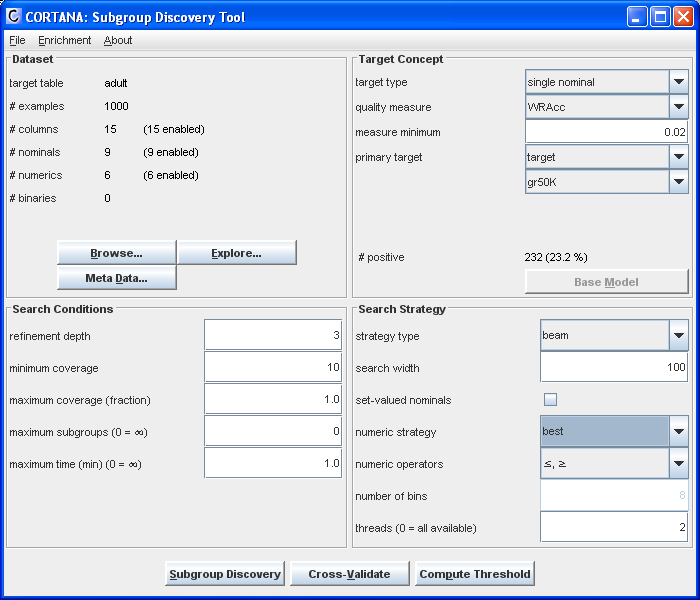
\includegraphics[width=\textwidth]{mainwindow.png}
\caption{Cortana's main window.}
\label{fig:mainwindow}
\end{center}
\end{figure}

The main screen of Cortana is devided into four major panels, \emph{Dataset}, \emph{Target Concept}, \emph{Search Conditions}, and \emph{Search Strategy}.

\subsection{Dataset Panel}

\begin{figure}
\begin{center}
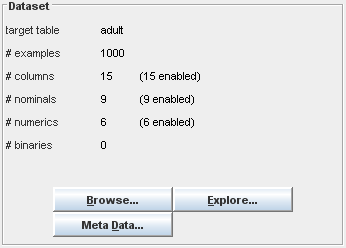
\includegraphics[width=0.5\textwidth]{dataset.png}
\caption{Dataset details in the main window.}
\end{center}
\label{fig:dataset}
\end{figure}

The dataset panel gives some information about the dataset that is currently loaded:
\begin{description}
\item[target table] shows the name of the data file used, which for text files is just the filename, and for ARFF files is the name defined in the '@relation' field;
\item[\# examples] shows the number of examples in the dataset;
\item[\# columns] shows the number of columns in the dataset.
Remember that columns are also be referred to as attributes.
\end{description}
Finally, there is a number of fields that indicate the number of attributes from each data type.
The type of an attribute determines the sort of mining algorithm or quality measure that is applicable to it.
More about this can be found in section~\ref{preliminaries:attribute-type}.

In addition to the fields described above, there are three buttons present on the {\bf Dataset} panel, {\bf Browse...}, {\bf Meta Data...} and {\bf Explore...}.

\subsubsection{Browse Window}

\begin{figure}
\begin{center}
\centering
\resizebox{1\columnwidth}{!}{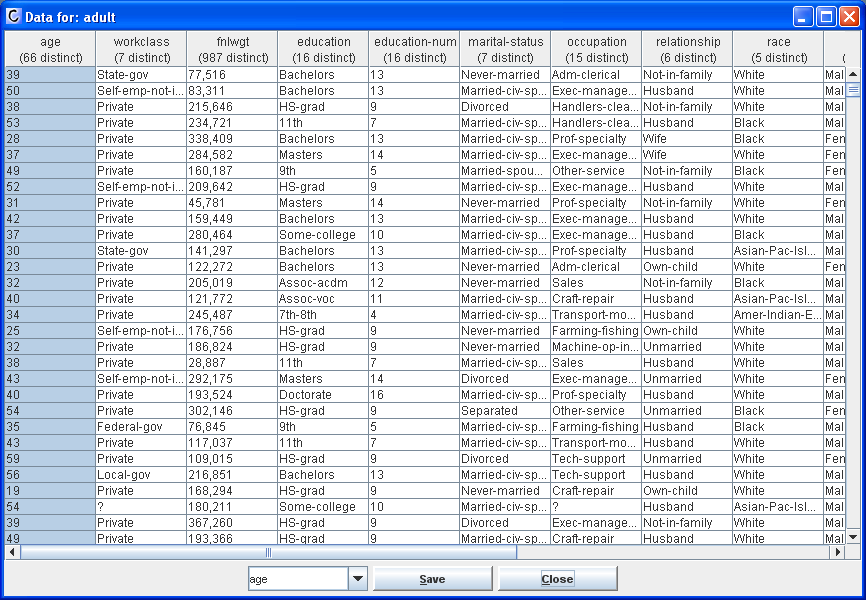
\includegraphics{browsewindow.png}}
\caption{The browse window.}
\end{center}
\label{fig:browsewindow}
\end{figure}

By clicking the {\bf Browse...} button, a Browse Window is presented, showing a table with the data in the state that it is currently in.
Additionally, in the table header, it shows the number of distinct values for each attribute.
Note that the data may not be in the same state as when it was loaded, as it can be modified using functionality of the Meta Data Window, presented after pressing the {\bf Meta Data...} button, which is also present on the {\bf Dataset} panel.
Section~\ref{sec:metadata} describes the Meta Data Window, its components, and the data manipulation functionalities, in more detail.

\subsubsection{Explore Window}

{\bf Explore...} button.

\subsubsection{Meta Data Window}
\label{sec:metadata}

\begin{figure}
\begin{center}
\centering
\resizebox{1\columnwidth}{!}{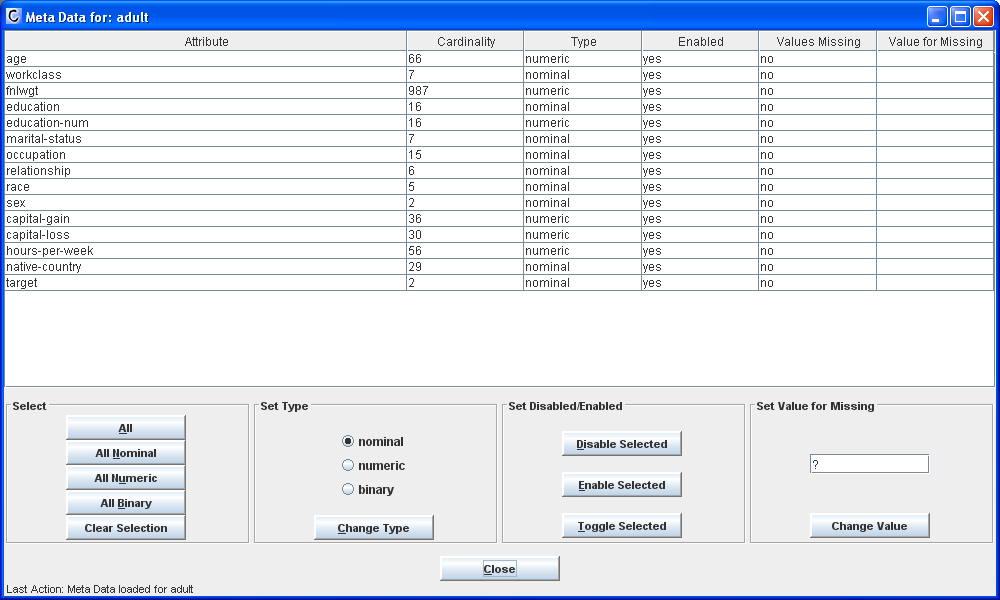
\includegraphics{metadatawindow.png}}
\caption{Meta data window.}
\end{center}
\label{fig:metadatawindow}
\end{figure}

The \textbf{Meta Data...} button gives access to a new window that, next to displaying some additional information about the dataset loaded, also allows changing some of the (characteristics of) the data.
The upper part of the \emph{Meta Data Window} shows a table with six columns.
The lower part contains a number of panels that allow modification of the data as it is in memory, note that no modifications are made to the original data file.
First the properties shown in the table in the upper part will be described, the purpose of the various data manipulations will be explained after that.

\paragraph{Meta Data Table}
\label{meta-data-window:meta-data-table}

The first column in this table, \emph{Attribute}, lists all \emph{attribute names} of the attributes in the dataset.
The remaining columns show some information for each of these attributes.
\emph{Cardiality} gives the number of distinct values for an attribute.
\emph{Type} shows its attribute type.
\emph{Enabled} indicates whether the attribute is \emph{enabled} or \emph{disabled}.
\emph{Values Missing} indicates whether the attribute contains missing values or not.
And finally, \emph{Missing Value} shows the value that is currently used for missing values in the data.
Obviously, this field is blank if there are no values missing for the attribute.

\paragraph{Meta Data Functions}
\label{meta-data-window:meta-data-functions}

The panels in the lower part of the \emph{Meta Data Window} all allow selecting or changing the data.
The first, \emph{Select}, allows selecting all attributes of a certain type.
This is a conveiniance method to be used in combination with the functionalities available in other panels.

\textbf{Set Type} allows changing the attribute type.
This can be useful for various reasons.
The first is that, after loading a plain text file, it is observed that Cortana was not capable to infer the correct type for an attribute.
Related to this is the possiblity to change the type of an attribute to allow other quality measures to be used in the Subgroup Discovery process.
An example of this would be an attribute that describes the number of doors in a car dataset.
If this value is used as a target value, one might treat it as a \emph{nominal} property, forcing the Subgroup Discovery process to only perform equality tests on this \emph{attribute value} for the creation of the conditions used to form subgroups.
\emph{Instances} in the dataset are then either in the target set if they have the same value for the `doors' attribute as the selected target value, or are in the complement of the set formed by those instances.
If the `doors' attribute is treated as \emph{numeric}, any, combination, of the `$<=$', `$>=$' and `$=$' tests can used to create conditions to perform on the \emph{attribute values}.
This means that the size of the set of instances selected using an \emph{attribute value} might be bigger than in the \emph{nominal} case.
A condition using $doors >= 2$ will select all cars having two or more doors.
In the \emph{nominal} case it would not be possible to select this group using only one condition (assuming the set of cars having more than two doors is not empty).
Obviously, it would be possible to select the same group using a set of conditions like $doors equals `2' \vee doors equals `3' \ldots$, but, among other negative characteristics, creating such conditions would be computationally more demanding, and less intuitive.
Note that if there are missing values for an attribute, the \emph{missing value} value for this attribute might be automaticaly changed to a value that is relevant to the attribute type.
See \emph{Set Value for Missing} below for more on the \emph{missing value} values for the different attribute types.
%\ref{subsubsection:set-missing-values}

\textbf{Set Disabled/Enabled} allows to disable or enable an attribute.
When an attribute is disabled, it will not be considered by the mining algorithm to form conditions with to create subgroups.
Note that disabling an attribute does not affect the possiblity to select it as a target concept (see section~\ref{preliminaries:target-concept} for more on target concepts).

\textbf{Set Value for Missing} can be used to change the value that is curently used for values that were missing in the data.
The value that is used for missing values depends on the type of the attribute.
If, in an ARFF file, values are declared missing, using the `\emph{?}' directive, Cortana's file loader might replace this value with one that makes more sense in its Subgroup Discovery setting.
For \emph{nominal} types it will leave this value as is.
This will result in `\emph{?}' being one of the possible target values one can select for the corresponding attribute.
However, one can assign a diffent value to the \emph{missing values}.
One than has two options, either assign the \emph{missing values} a value that is an existing one for the attribute, or a non-exiting one.
In the first case one effectively assigns all instances that have a missing value for the corresponding attribute to one of the other \emph{attribute values}.
In the latter case, one just changes the value.
When changing the \emph{missing value} value of an attribute, the \emph{Cardinality} column is updated accordingly.
For \emph{numeric} and \emph{binary} attribute types Cortana's file loader will replace `\emph{?}' values with $0.0$ and $false$, respectively.
Again, if this is incorrect, or one wishes to assign the \emph{missing values} another \emph{attribute value}, either existing or non-existing, this can be done analogously to the \emph{nominal} case.

\subsection{Target Concept Panel}

\subsection{Search Conditions Panel}

\subsection{Search Strategy Panel}

\section{Result Window}

\appendix
\clearpage
~\vfill

\resizebox{\textwidth}{!}{Appendices}

\vfill~
\clearpage

\section{Glossary}

\section{Autorun}

\section{Memory Issues}
\label{sec:memory}

Although Cortana is written in Java, and therefore platform independent, it will behave slightly different on different operation systems and/or platforms.
These differences arise from small variations in the Java Virtual Machines, used in different situations.
The main issue is with 32-bit operating systems (OS).
On such systems the maximum amount of memory the Java Virtual Machine (JVM) can use is around 1600 MegaBytes.
However, the actual amount depends on the amount of RAM available.
The cortana.bat and cortana.sh file included in the Cortana.zip set the maximum amount of memory the JVM can use to 1600 MegaBytes, through the -Xmx option.
The value should, at most, be set to half the amount of available RAM, meaning eg. for a 2GB machine to \emph{-Xmx1000m}.
For 64-bit OSes no such limit exists, and it should be save to remove the -Xmx.
Note that the above means that, especially for 32-bit OSes, not all datasets will fit into memory.

\end{document}
